% Options for packages loaded elsewhere
\PassOptionsToPackage{unicode}{hyperref}
\PassOptionsToPackage{hyphens}{url}
\PassOptionsToPackage{dvipsnames,svgnames,x11names}{xcolor}
%
\documentclass[
  letterpaper,
  DIV=11,
  numbers=noendperiod]{scrartcl}

\usepackage{amsmath,amssymb}
\usepackage{iftex}
\ifPDFTeX
  \usepackage[T1]{fontenc}
  \usepackage[utf8]{inputenc}
  \usepackage{textcomp} % provide euro and other symbols
\else % if luatex or xetex
  \usepackage{unicode-math}
  \defaultfontfeatures{Scale=MatchLowercase}
  \defaultfontfeatures[\rmfamily]{Ligatures=TeX,Scale=1}
\fi
\usepackage{lmodern}
\ifPDFTeX\else  
    % xetex/luatex font selection
\fi
% Use upquote if available, for straight quotes in verbatim environments
\IfFileExists{upquote.sty}{\usepackage{upquote}}{}
\IfFileExists{microtype.sty}{% use microtype if available
  \usepackage[]{microtype}
  \UseMicrotypeSet[protrusion]{basicmath} % disable protrusion for tt fonts
}{}
\makeatletter
\@ifundefined{KOMAClassName}{% if non-KOMA class
  \IfFileExists{parskip.sty}{%
    \usepackage{parskip}
  }{% else
    \setlength{\parindent}{0pt}
    \setlength{\parskip}{6pt plus 2pt minus 1pt}}
}{% if KOMA class
  \KOMAoptions{parskip=half}}
\makeatother
\usepackage{xcolor}
\setlength{\emergencystretch}{3em} % prevent overfull lines
\setcounter{secnumdepth}{-\maxdimen} % remove section numbering
% Make \paragraph and \subparagraph free-standing
\ifx\paragraph\undefined\else
  \let\oldparagraph\paragraph
  \renewcommand{\paragraph}[1]{\oldparagraph{#1}\mbox{}}
\fi
\ifx\subparagraph\undefined\else
  \let\oldsubparagraph\subparagraph
  \renewcommand{\subparagraph}[1]{\oldsubparagraph{#1}\mbox{}}
\fi


\providecommand{\tightlist}{%
  \setlength{\itemsep}{0pt}\setlength{\parskip}{0pt}}\usepackage{longtable,booktabs,array}
\usepackage{calc} % for calculating minipage widths
% Correct order of tables after \paragraph or \subparagraph
\usepackage{etoolbox}
\makeatletter
\patchcmd\longtable{\par}{\if@noskipsec\mbox{}\fi\par}{}{}
\makeatother
% Allow footnotes in longtable head/foot
\IfFileExists{footnotehyper.sty}{\usepackage{footnotehyper}}{\usepackage{footnote}}
\makesavenoteenv{longtable}
\usepackage{graphicx}
\makeatletter
\def\maxwidth{\ifdim\Gin@nat@width>\linewidth\linewidth\else\Gin@nat@width\fi}
\def\maxheight{\ifdim\Gin@nat@height>\textheight\textheight\else\Gin@nat@height\fi}
\makeatother
% Scale images if necessary, so that they will not overflow the page
% margins by default, and it is still possible to overwrite the defaults
% using explicit options in \includegraphics[width, height, ...]{}
\setkeys{Gin}{width=\maxwidth,height=\maxheight,keepaspectratio}
% Set default figure placement to htbp
\makeatletter
\def\fps@figure{htbp}
\makeatother
% definitions for citeproc citations
\NewDocumentCommand\citeproctext{}{}
\NewDocumentCommand\citeproc{mm}{%
  \begingroup\def\citeproctext{#2}\cite{#1}\endgroup}
\makeatletter
 % allow citations to break across lines
 \let\@cite@ofmt\@firstofone
 % avoid brackets around text for \cite:
 \def\@biblabel#1{}
 \def\@cite#1#2{{#1\if@tempswa , #2\fi}}
\makeatother
\newlength{\cslhangindent}
\setlength{\cslhangindent}{1.5em}
\newlength{\csllabelwidth}
\setlength{\csllabelwidth}{3em}
\newenvironment{CSLReferences}[2] % #1 hanging-indent, #2 entry-spacing
 {\begin{list}{}{%
  \setlength{\itemindent}{0pt}
  \setlength{\leftmargin}{0pt}
  \setlength{\parsep}{0pt}
  % turn on hanging indent if param 1 is 1
  \ifodd #1
   \setlength{\leftmargin}{\cslhangindent}
   \setlength{\itemindent}{-1\cslhangindent}
  \fi
  % set entry spacing
  \setlength{\itemsep}{#2\baselineskip}}}
 {\end{list}}
\usepackage{calc}
\newcommand{\CSLBlock}[1]{\hfill\break\parbox[t]{\linewidth}{\strut\ignorespaces#1\strut}}
\newcommand{\CSLLeftMargin}[1]{\parbox[t]{\csllabelwidth}{\strut#1\strut}}
\newcommand{\CSLRightInline}[1]{\parbox[t]{\linewidth - \csllabelwidth}{\strut#1\strut}}
\newcommand{\CSLIndent}[1]{\hspace{\cslhangindent}#1}

\KOMAoption{captions}{tableheading}
\makeatletter
\@ifpackageloaded{caption}{}{\usepackage{caption}}
\AtBeginDocument{%
\ifdefined\contentsname
  \renewcommand*\contentsname{Table of contents}
\else
  \newcommand\contentsname{Table of contents}
\fi
\ifdefined\listfigurename
  \renewcommand*\listfigurename{List of Figures}
\else
  \newcommand\listfigurename{List of Figures}
\fi
\ifdefined\listtablename
  \renewcommand*\listtablename{List of Tables}
\else
  \newcommand\listtablename{List of Tables}
\fi
\ifdefined\figurename
  \renewcommand*\figurename{Figure}
\else
  \newcommand\figurename{Figure}
\fi
\ifdefined\tablename
  \renewcommand*\tablename{Table}
\else
  \newcommand\tablename{Table}
\fi
}
\@ifpackageloaded{float}{}{\usepackage{float}}
\floatstyle{ruled}
\@ifundefined{c@chapter}{\newfloat{codelisting}{h}{lop}}{\newfloat{codelisting}{h}{lop}[chapter]}
\floatname{codelisting}{Listing}
\newcommand*\listoflistings{\listof{codelisting}{List of Listings}}
\makeatother
\makeatletter
\makeatother
\makeatletter
\@ifpackageloaded{caption}{}{\usepackage{caption}}
\@ifpackageloaded{subcaption}{}{\usepackage{subcaption}}
\makeatother
\ifLuaTeX
  \usepackage{selnolig}  % disable illegal ligatures
\fi
\usepackage{bookmark}

\IfFileExists{xurl.sty}{\usepackage{xurl}}{} % add URL line breaks if available
\urlstyle{same} % disable monospaced font for URLs
\hypersetup{
  pdftitle={Predicting the Price of New York City Airbnbs (DSCI 310 Group 9)},
  pdfauthor={Oliver Gullery, Prithvi Sureka, Rashi Selarka \& Riddhi Battu},
  colorlinks=true,
  linkcolor={blue},
  filecolor={Maroon},
  citecolor={Blue},
  urlcolor={Blue},
  pdfcreator={LaTeX via pandoc}}

\title{Predicting the Price of New York City Airbnbs (DSCI 310 Group 9)}
\author{Oliver Gullery, Prithvi Sureka, Rashi Selarka \& Riddhi Battu}
\date{}

\begin{document}
\maketitle

\renewcommand*\contentsname{Table of contents}
{
\hypersetup{linkcolor=}
\setcounter{tocdepth}{2}
\tableofcontents
}
\section{Summary}\label{summary}

We are developing a classification model using a KNN machine learning
algorithm to categorize Airbnb listing prices into various ranges. The
goal is to accurately assign each listing to a price bracket, starting
at \$0 and increasing in \$50 increments up to \$350 and above. The
classifier is designed to help potential guests estimate the price range
of a rental before detailed information is provided. The performance of
our model on the test data set indicates varying degrees of precision
and recall across different price categories, with an overall accuracy
of 0.51. Given that the data set consists of 7926 instances, the model
shows promise, but there is significant room for improvement. Particular
attention should be given to enhancing the performance for categories
that currently show lower F1-scores. Further analysis is needed to
understand the features that most affect price prediction accuracy and
to refine the model for better performance across all price ranges.

\section{Introduction}\label{introduction}

Airbnb has been one of the most popular short-term stays and rental
online services since 2008, expanding to over a thousand cities in less
than a year (Geron 2009). Owing to its exponential growth however, many
metropolises such as Paris, London, Berlin, and New York City started
introducing special rules and laws for creating a listing on Airbnb due
to its impact on housing shortages and rental markets (Tun 2023). In
September 2023, New York enforced a measure called Local Law 18 (Oladipo
2023), that was essentially a de facto ban on short-term rentals that
would force the amount of listings to decrease 85\% within the month
(Chan 2023), and decrease over 90\% as of 2024 from what they were in
2022 (Bellafante 2024). Consequently, this led average prices to surge,
and led us to want to investigate factors of New York Airbnbs and how
they impact listing prices.

We were able to obtain a workable and descriptive dataset about New York
Airbnbs from
\href{http://insideairbnb.com/new-york-city/}{insideairbnb.com} (Inside
Airbnb 2024) that gave insight into every listing from 2011 to 2023 and
their reviews. The fields present in our dataset are:

\begin{itemize}
\tightlist
\item
  ID: Unique identifier for listing
\item
  Name: Name of listing, followed by rating and type (e.g.~1 bed 1 bath)
\item
  Host ID: Unique identifier for host
\item
  Host Name: Name of host
\item
  Neighbourhood: Neighbourhood where listing is located
\item
  Neighbourhood Group: Borough where listing is located
\item
  Latitude: Latitudinal coordinate of listing location
\item
  Longitude: Longitudinal coordinate of listing location
\item
  Room Type: Listing space type (Private room, Entire home / Apt., etc.)
\item
  Price: Price per Night in USD
\item
  Minimum Nights: Minimum nights required to stay at the rental
\item
  Number of Reviews: Total number of reviews on the listing
\item
  Last Review: Date of latest review on the rental
\item
  Reviews Per Month: Avg. monthly number of reviews on the listing
\item
  Calculated Host Listings Count: Number of listings the corresponding
  host has
\item
  Availability 365: Number of days in a year listing is available for
  booking
\end{itemize}

Here we intend to use a machine learning algorithm to predict Airbnb
prices per night using most of the above factors. There have been
multiple studies looking into how the Airbnb ban impacts NYC rental
(Fields 2023) and hotel prices (Kelly 2023), but not as much into the
Airbnb prices themselves. Since our investigation will be solely based
on data up until 2023, it can be used glean exactly how these
restrictions impacted Airbnb prices in NYC when compared with
information from 2024 onwards (i.e.~was it because the number of
listings per host went down? Or was it because the minimum number of
nights required to stay went up? and more questions like that). As
Airbnb prices can range to various amounts, we will look to \emph{bin
prices into different categories in increments of 50}. This will help us
provide a more accurate range of price recommendations when looking at
different Airbnb listings

\section{Methods}\label{methods}

The Python programming language (Van Rossum and Drake 2009) and the
following Python packages were primarily used to perform the analysis:
pandas (McKinney 2010), scikitlearn (Pedregosa et al. 2011), click (Team
2020), as well as Quarto (Allaire et al. 2022).

As previously mentioned, we loaded data from
\href{http://insideairbnb.com/new-york-city/}{insideairbnb.com} (Inside
Airbnb 2024).

\subsection{Takeaways From Preliminary
EDA}\label{takeaways-from-preliminary-eda}

\begin{itemize}
\item
  We have 39627 rows and 18 features which includes \texttt{price}. We
  decided it was a good idea to generate a \texttt{price\_category}
  variable as our target variable that classified the price into bins /
  brackets starting at \$0 and increasing in \$50 increments up to \$350
  +.
\item
  We identified that \texttt{name} is text type data which could provide
  some valuable insights. We can also infer that any id information
  (\texttt{id} and \texttt{host\_id}) and variables such as
  \texttt{host\_name} will not provide any key information, thus, we can
  drop them for our data analysis.
\item
  The column \texttt{host\_name} had \emph{15} null values but it is not
  a roadblock since we dropped this column. Our
  \texttt{reviews\_per\_month} column and \texttt{last\_review} column
  have \emph{11480} null values each. This suggests that when a airbnb
  listing doesn't have a review, it was listed as a null value in the
  data. To fix this we could impute 0 into the nulls for
  \texttt{reviews\_per\_month}. For \texttt{last\_review}, we decided it
  would be appropriate to drop the column as some of the information it
  provides is stored in reviews per month.
\item
  \texttt{license} has a significant number of null values with 35268.
  It might provide some interesting insights into price as a license is
  proof that the airbnb owners comply with the regulatory standards, but
  since the nature of these missing values is unknown, we cannot be sure
  if the null values means the listing has no license. Due to this
  imbalance in the data, we decided it best to drop this column.
  However, it could be worth exploring the relationship between license
  and other variables in future analyses.
\end{itemize}

\subsection{Next Steps for Feature
Engineering}\label{next-steps-for-feature-engineering}

In order to prepare our data for further analysis we performed some
preliminary feature engineering: - Converted \texttt{id} and
\texttt{host\_id} into object datatypes to prepare them to be dropped. -
Imputed zeros into the \texttt{reviews\_per\_month} null values. -
Segregated fields into target column, categorical, numerical, text data,
and drop data. - Created a price category variable.

After this cleaning, we split the data into training and test sets.

\subsection{\texorpdfstring{Spread of \texttt{price}
Visualized}{Spread of price Visualized}}\label{spread-of-price-visualized}

We plotted a histogram for our \texttt{price} variable to graph its'
spread on Figure~\ref{fig-price-plot} below.

\begin{figure}[H]

\centering{

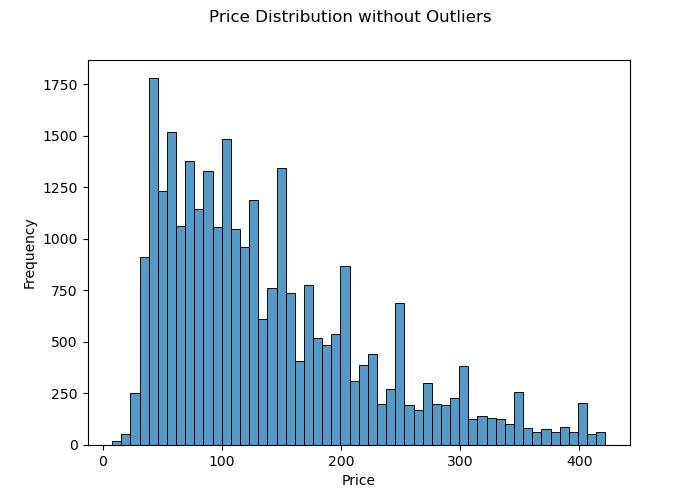
\includegraphics[width=0.8\textwidth,height=\textheight]{../results/figures/price_histogram.jpg}

}

\caption{\label{fig-price-plot}Price Histogram (Outliers Removed).}

\end{figure}%

\subsection{Relationships between Predictors
Visualized}\label{relationships-between-predictors-visualized}

We examined the correlations between the numeric data we had present to
help us understand which predictors could be used in tandem. The top 10
crorrelations are displayed in Table~\ref{tbl-corr-ranked} below, and we
plotted a correlation heat map on Figure~\ref{fig-corr-plot} to
visualize it:

\begin{longtable}[]{@{}
  >{\raggedright\arraybackslash}p{(\columnwidth - 4\tabcolsep) * \real{0.4051}}
  >{\raggedright\arraybackslash}p{(\columnwidth - 4\tabcolsep) * \real{0.4051}}
  >{\raggedleft\arraybackslash}p{(\columnwidth - 4\tabcolsep) * \real{0.1899}}@{}}

\caption{\label{tbl-corr-ranked}Top 10 Correlations Ranked.}

\tabularnewline

\toprule\noalign{}
\begin{minipage}[b]{\linewidth}\raggedright
Variable\_1
\end{minipage} & \begin{minipage}[b]{\linewidth}\raggedright
Variable\_2
\end{minipage} & \begin{minipage}[b]{\linewidth}\raggedleft
Correlation
\end{minipage} \\
\midrule\noalign{}
\endhead
\bottomrule\noalign{}
\endlastfoot
reviews\_per\_month & number\_of\_reviews\_ltm & 0.864186 \\
reviews\_per\_month & number\_of\_reviews & 0.68403 \\
number\_of\_reviews & number\_of\_reviews\_ltm & 0.649095 \\
id & host\_id & 0.467509 \\
id & availability\_365 & 0.339904 \\
availability\_365 & host\_id & 0.269954 \\
id & number\_of\_reviews & -0.220865 \\
calculated\_host\_listings\_count & id & 0.170879 \\
host\_id & reviews\_per\_month & 0.139133 \\
availability\_365 & calculated\_host\_listings\_count & 0.136801 \\

\end{longtable}

\begin{figure}[H]

\centering{

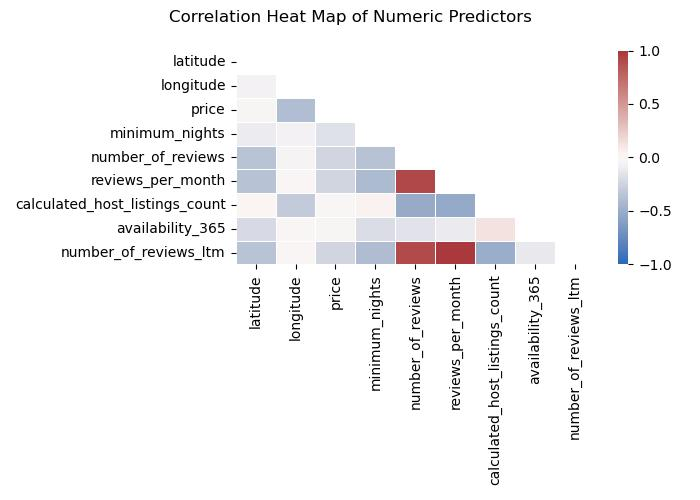
\includegraphics[width=0.8\textwidth,height=\textheight]{../results/figures/corr_heat_map.jpg}

}

\caption{\label{fig-corr-plot}Correlation Heat Map of Numerical
Predictors of Airbnb Price.}

\end{figure}%

We see from Figure~\ref{fig-corr-plot} that
\texttt{number\_of\_reviews}, \texttt{reviews\_per\_month}, and
\texttt{number\_of\_reviews\_ltm} appear to have the strongest
correlations between them, indicating they interact with each other
more.

We also visualized the relationships between some of our other
predictors to view the spread of our data and the impact of every
predictor on \texttt{price} (to extend it to the impact it has on
\texttt{price\ category}).

We plotted the physical location by latitude and longitude of every
listing on Figure~\ref{fig-location-plot}, placed alongside an outline
of a map of NYC to see the concentration of listings between boroughs.

\begin{figure}[H]

\centering{

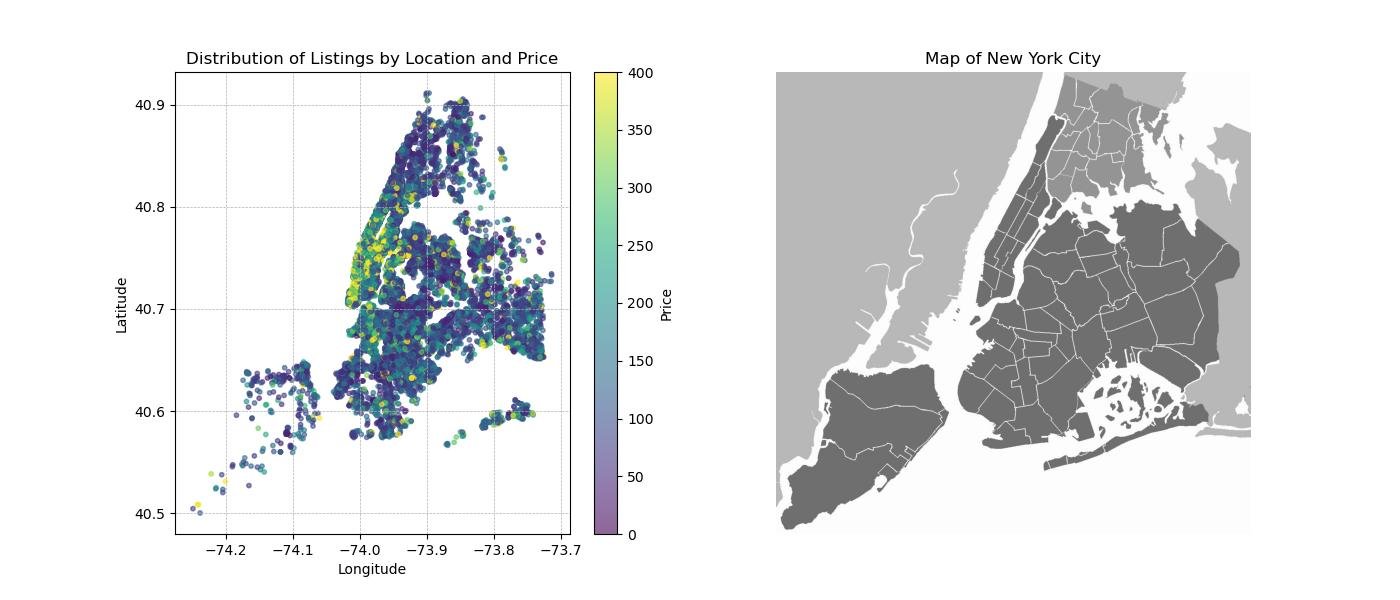
\includegraphics{../results/figures/listing_locations.jpg}

}

\caption{\label{fig-location-plot}Map with Distribution of Listings by
Location and Price.}

\end{figure}%

We also created scatterplots of \texttt{price} against the
\texttt{number\_of\_reviews} as well as the \texttt{reviews\_per\_month}
on Figure~\ref{fig-price-v-reviews-plot} and
Figure~\ref{fig-price-v-reviews-per-month-plot} respectively to
understand how the distribution compares for the two - considering both
predictors were largely correlated with each other.

\begin{figure}[H]

\centering{

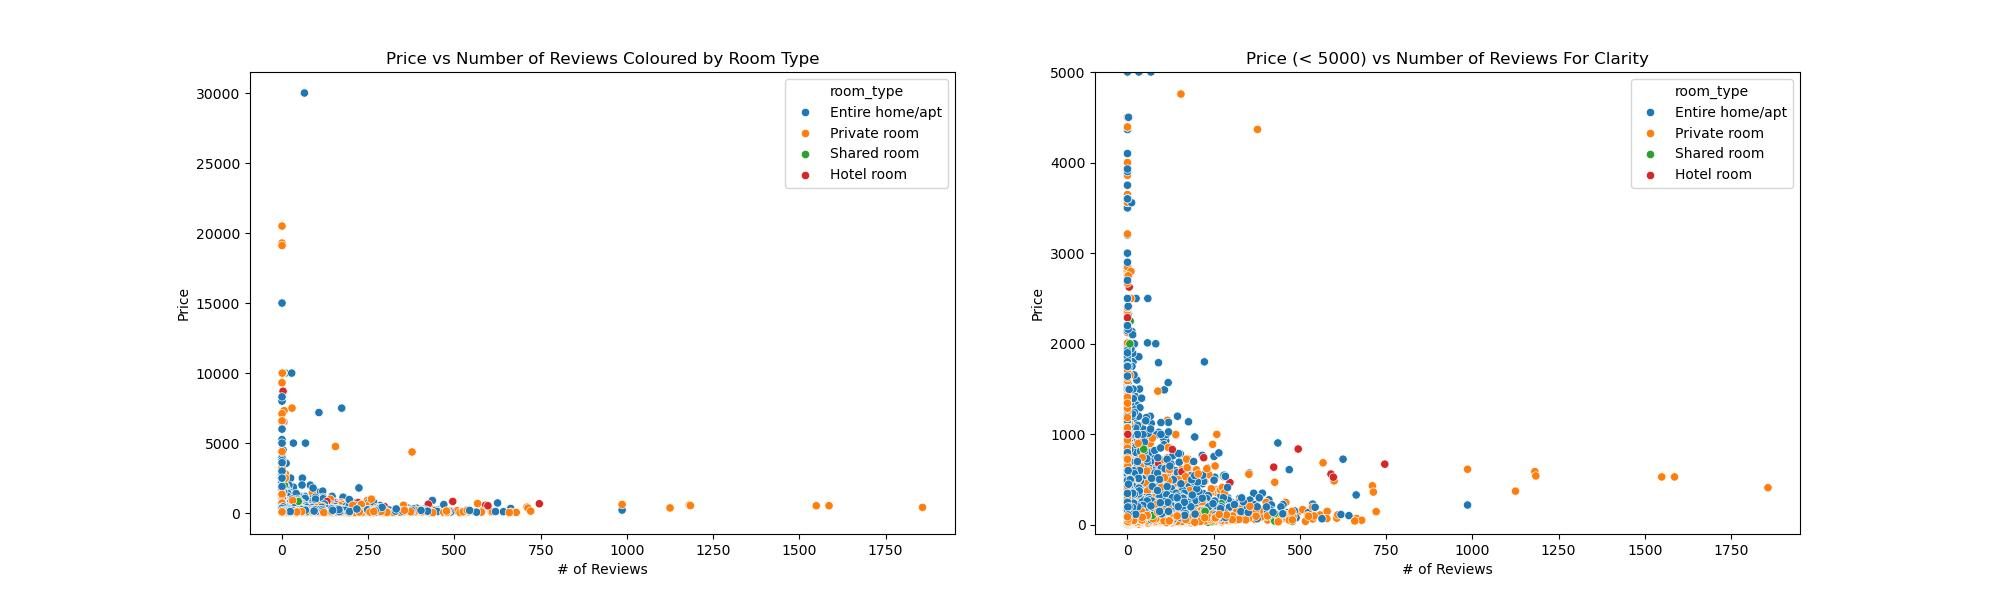
\includegraphics{../results/figures/price_vs_reviews.jpg}

}

\caption{\label{fig-price-v-reviews-plot}Price vs Number of Reviews
Coloured by Room Type Scatterplot.}

\end{figure}%

\begin{figure}[H]

\centering{

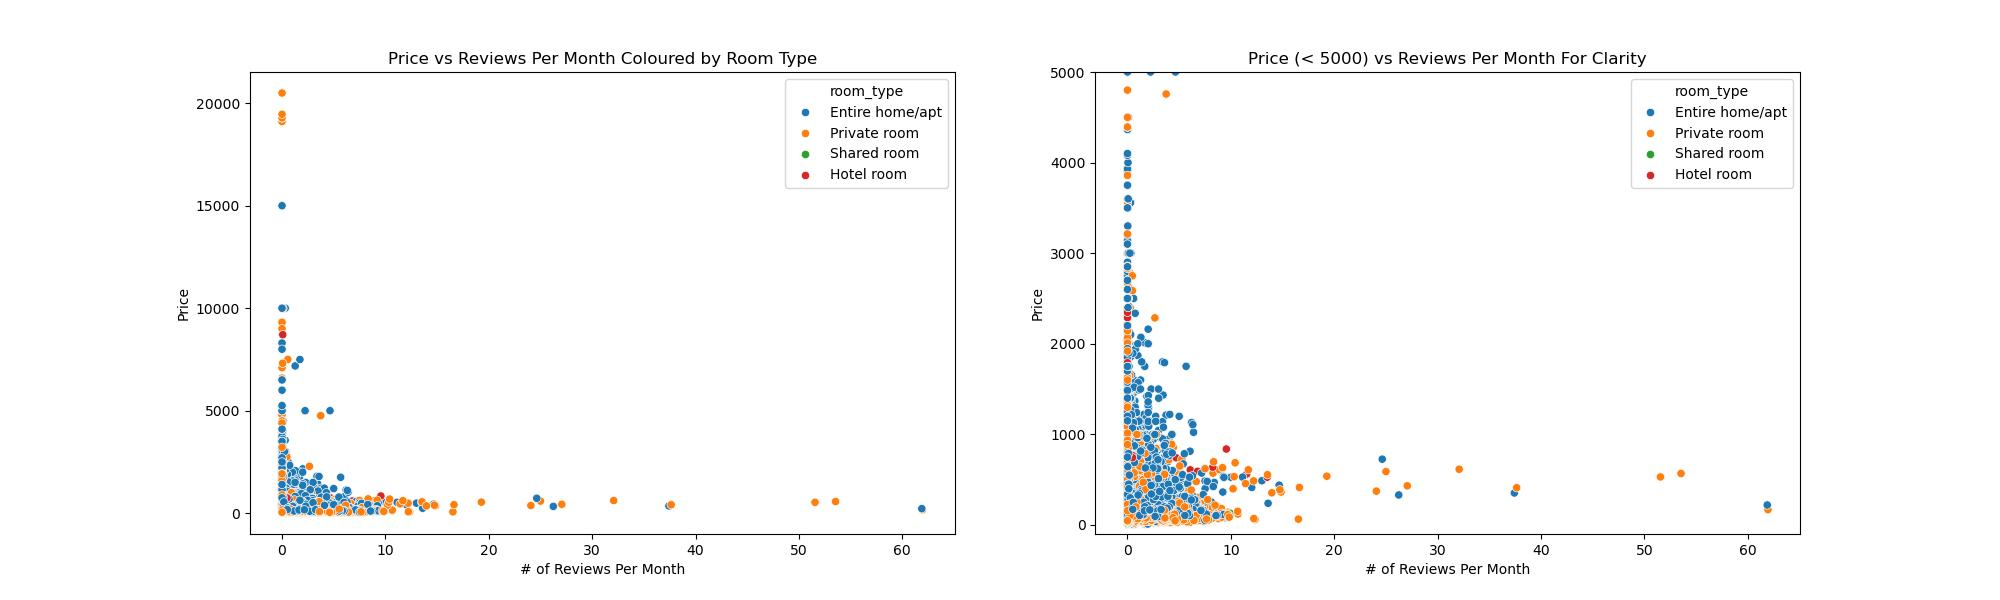
\includegraphics{../results/figures/price_vs_reviews_per_month.jpg}

}

\caption{\label{fig-price-v-reviews-per-month-plot}Price vs Reviews Per
Month Coloured by Room Type Scatterplot.}

\end{figure}%

We then created side-by-side boxplots to compare \texttt{price} (as well
as log price for clarity) against the \texttt{neighbourhood\_group} or
the NYC borough, as well as \texttt{room\_type} to view the isolated
relationships between price and those 2 predictors and the spread of the
listings in each category. They can be see in
Figure~\ref{fig-neighbourhood-plot} and Figure~\ref{fig-room-type-plot}
below:

\begin{figure}[H]

\centering{

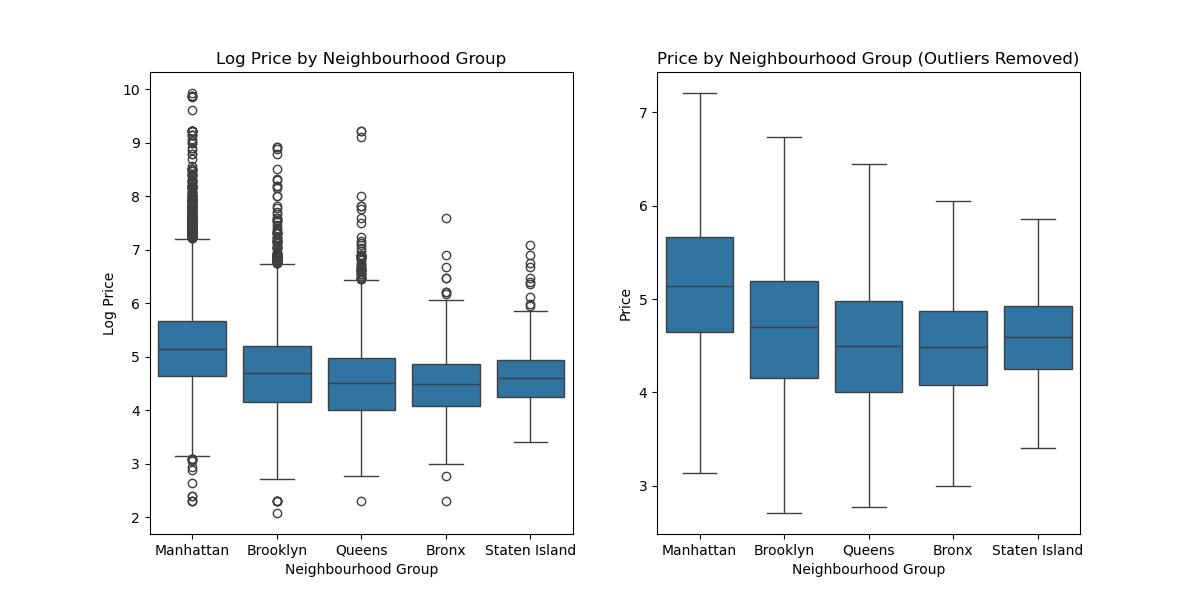
\includegraphics{../results/figures/neighbourhood_groups_boxplots.jpg}

}

\caption{\label{fig-neighbourhood-plot}Log Price and Price by
Neighbourhood Group Boxplot.}

\end{figure}%

\begin{figure}[H]

\centering{

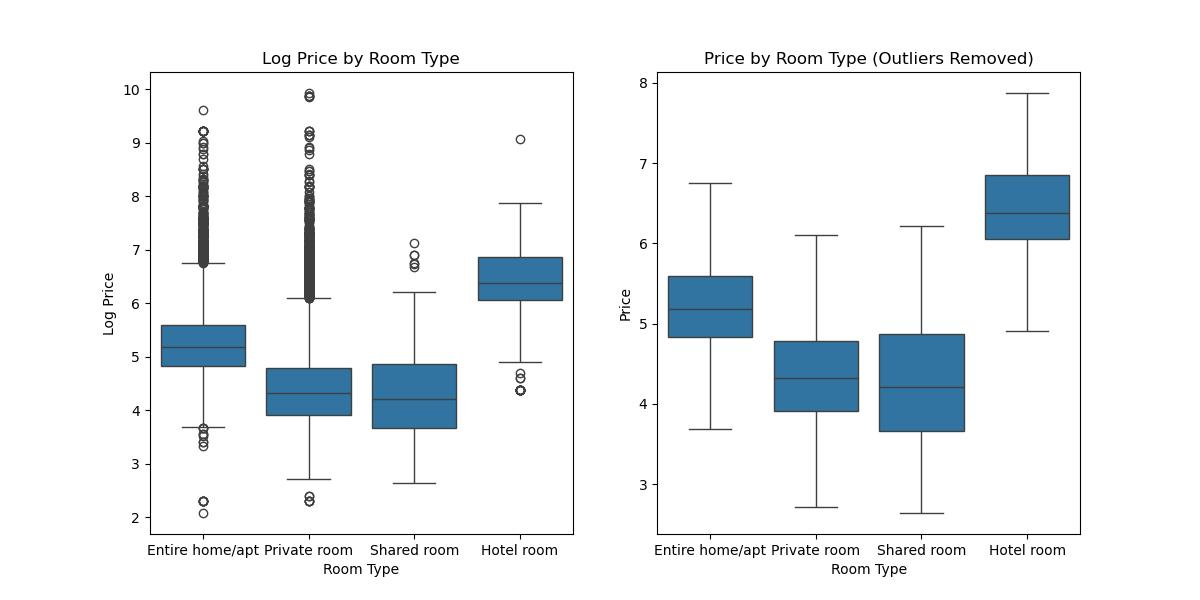
\includegraphics{../results/figures/room_type_boxplots.jpg}

}

\caption{\label{fig-room-type-plot}Log Price and Price by Room Type
Boxplot.}

\end{figure}%

After this, we moved onto creating our preprocessor and model.

\subsection{Defining Transformations and
Model}\label{defining-transformations-and-model}

We defined transformations on our data, using \texttt{StandardScaler} on
our numerical data, \texttt{OneHotEncoder} on our categorical data,
\texttt{CountVectorizer} on our text data. We also implement a Dummy
Regressor model as a baseline to assess our model with.

We then proceed to fit a K-Nearest-Neighbours Classification model using
\texttt{KNeighborsClassifier} from (Pedregosa et al. 2011).

\subsection{Re-evaluating Model with Hyperparameter
Optimization}\label{re-evaluating-model-with-hyperparameter-optimization}

We decided to also use \texttt{RandomizedSearchCV} to choose
hyperparameters that would yield an optimal model for our data.

\section{Results}\label{results}

We generated classification reports for all 3 models we fit - the Dummy
regressor, the original KNN and the KNN after hyperparameter
optimization to compare their performance and accuracy.

\subsection{Classification Report for Dummy
Model}\label{classification-report-for-dummy-model}

\begin{longtable}[]{@{}lrrrr@{}}

\caption{\label{tbl-dummy-clf}Classification Report for Dummy
Regressor.}

\tabularnewline

\toprule\noalign{}
Criterion & precision & recall & f1-score & support \\
\midrule\noalign{}
\endhead
\bottomrule\noalign{}
\endlastfoot
0-50 & 0 & 0 & 0 & 1061 \\
50-100 & 0.266843 & 1 & 0.421273 & 2115 \\
100-150 & 0 & 0 & 0 & 1640 \\
150-200 & 0 & 0 & 0 & 1077 \\
200-250 & 0 & 0 & 0 & 576 \\
250-300 & 0 & 0 & 0 & 397 \\
300-350 & 0 & 0 & 0 & 224 \\
350+ & 0 & 0 & 0 & 836 \\
accuracy & 0.266843 & 0.266843 & 0.266843 & 0.266843 \\
macro avg & 0.0333554 & 0.125 & 0.0526591 & 7926 \\
weighted avg & 0.0712053 & 0.266843 & 0.112414 & 7926 \\

\end{longtable}

We see in Table~\ref{tbl-dummy-clf} here that the accuracy for the dummy
model is 0.27.

\subsection{Classification Report for KNN
Model}\label{classification-report-for-knn-model}

\begin{longtable}[]{@{}lrrrr@{}}

\caption{\label{tbl-knn-clf}Classification Report for KNN Classification
Model.}

\tabularnewline

\toprule\noalign{}
Criterion & precision & recall & f1-score & support \\
\midrule\noalign{}
\endhead
\bottomrule\noalign{}
\endlastfoot
0-50 & 0.599291 & 0.637135 & 0.617634 & 1061 \\
50-100 & 0.508475 & 0.638298 & 0.566038 & 2115 \\
100-150 & 0.400713 & 0.410976 & 0.40578 & 1640 \\
150-200 & 0.317719 & 0.289694 & 0.30306 & 1077 \\
200-250 & 0.224 & 0.145833 & 0.176656 & 576 \\
250-300 & 0.232 & 0.146096 & 0.179289 & 397 \\
300-350 & 0.205357 & 0.102679 & 0.136905 & 224 \\
350+ & 0.645553 & 0.572967 & 0.607098 & 836 \\
accuracy & 0.461267 & 0.461267 & 0.461267 & 0.461267 \\
macro avg & 0.391638 & 0.367959 & 0.374057 & 7926 \\
weighted avg & 0.443784 & 0.461267 & 0.448585 & 7926 \\

\end{longtable}

We see in Table~\ref{tbl-knn-clf} here that the accuracy for the KNN
model is 0.46, which is better than our dummy model, but we still want
to see if we can do better with another choice of neighbours. Upon
hyperparameter optimization, we found that 15 neighbours proved to be
the optimal choice.

\subsection{Classification Report After Hyperparameter
Optimization}\label{classification-report-after-hyperparameter-optimization}

\begin{longtable}[]{@{}lrrrr@{}}

\caption{\label{tbl-hyperparam-clf}Classification Report for KNN after
Hyperparameter Optimization.}

\tabularnewline

\toprule\noalign{}
Criterion & precision & recall & f1-score & support \\
\midrule\noalign{}
\endhead
\bottomrule\noalign{}
\endlastfoot
0-50 & 0.684211 & 0.600377 & 0.639558 & 1061 \\
50-100 & 0.543624 & 0.689362 & 0.60788 & 2115 \\
100-150 & 0.411232 & 0.415244 & 0.413228 & 1640 \\
150-200 & 0.326087 & 0.320334 & 0.323185 & 1077 \\
200-250 & 0.245902 & 0.15625 & 0.191083 & 576 \\
250-300 & 0.315315 & 0.176322 & 0.226171 & 397 \\
300-350 & 0.29703 & 0.133929 & 0.184615 & 224 \\
350+ & 0.617582 & 0.672249 & 0.643757 & 836 \\
accuracy & 0.488645 & 0.488645 & 0.488645 & 0.488645 \\
macro avg & 0.430123 & 0.395508 & 0.403685 & 7926 \\
weighted avg & 0.47325 & 0.488645 & 0.475573 & 7926 \\

\end{longtable}

From Table~\ref{tbl-hyperparam-clf} we see that this optimization
processes improved the accuracy of our model from around 0.46 to 0.49.

\section{Discussion}\label{discussion}

Our investigation utilized an KNN machine learning algorithm to estimate
pricing categories for Airbnb listings in New York City. The dataset was
divided using an 80/20 train-test split, and we processed features as
either numerical or categorical to forecast the prices within
predetermined ranges. The model achieved an accuracy of about 0.49 as
indicated in the classification report above, which is not the best
however, considering the complexity of the pricing structure in the
short-term rental market it performed decently.

The level of accuracy attained was anticipated to some extent. We
undertook a meticulous selection of predictive variables and addressed
missing values to enhance the model's precision. However, the modest
F1-score indicates the model could benefit from improvements such as
better feature selection and feature engineering. This could be done
through performing feature importance analysis and working with that
information to further develop our model. We created a model with a KNN
to test.

At present, our feature importance metrics may be distorted due to the
numerous variables generated through one-hot encoding. For subsequent
analyses, we might consider exploring alternative methods to evaluate
feature significance, such as aggregating the importance of dummy
variables back to the original categorical variables, or employing
encoding techniques that preserve more information about the categorical
variable's cardinality and inherent ordering. This approach could
potentially provide a more accurate reflection of each feature's true
contribution to the predictive model.

The implications of such a model are significant. For renters, it could
mean a more informed decision-making process, as they could benchmark
individual rental prices against the broader market. Landlords might
utilize the model to set competitive prices, ensuring their offerings
are in line with current market conditions.

Moving forward, this study opens up several avenues for further inquiry.
One such area is the incorporation of temporal dynamics into the model,
as pricing could be influenced by seasonal trends or significant events.
Continuous refinement of the model is essential to maintain its
relevance, as the short-term rental market is subject to frequent
fluctuations. Additionally, investigating the outliers and misclassified
instances could provide insights into the limitations of the current
model and guide enhancements in predictive accuracy.

\section*{References}\label{references}
\addcontentsline{toc}{section}{References}

\phantomsection\label{refs}
\begin{CSLReferences}{1}{0}
\bibitem[\citeproctext]{ref-Allaire_Quarto_2022}
Allaire, J. J., Charles Teague, Carlos Scheidegger, Yihui Xie, and
Christophe Dervieux. 2022. {``{Quarto}.''}
\url{https://doi.org/10.5281/zenodo.5960048}.

\bibitem[\citeproctext]{ref-Bellafante_2024}
Bellafante, Ginia. 2024. {``Can a New Law Force Airbnb Hosts to Become
Landlords?''} \emph{The New York Times}, February.
\url{https://www.nytimes.com/2024/02/09/nyregion/nyc-airbnb-rentals.html}.

\bibitem[\citeproctext]{ref-Chan_2023}
Chan, Wilfred. 2023. {``'We're in a Housing Desert': A Month in, Is New
York's Airbnb Crackdown Working?''} \emph{The Guardian}, October.
\url{https://www.theguardian.com/us-news/2023/oct/23/new-york-airbnb-crackdown-rules-housing}.

\bibitem[\citeproctext]{ref-Fields_2023}
Fields, Samantha. 2023. {``Can an Airbnb Crackdown Really Make New York
More Affordable?''} \emph{Marketplace}.
\url{https://www.marketplace.org/2023/08/24/new-york-city-airbnb-crackdown-affordable-housing/}.

\bibitem[\citeproctext]{ref-Geron_2009}
Geron, Tomio. 2009. {``From Crash Pad to Pizza Profitable, Start-up Eyes
Budget Travel Market.''} \emph{The Wall Street Journal}, June.
\url{https://www.wsj.com/articles/BL-VCDB-2042}.

\bibitem[\citeproctext]{ref-New_York_City}
Inside Airbnb. 2024. {``Inside Airbnb: New York City.''}
\emph{Marketplace}. Inside Airbnb - Open Data.
\url{http://insideairbnb.com/new-york-city}.

\bibitem[\citeproctext]{ref-Kelly_2023}
Kelly, Griffin. 2023. {``New York City's Airbnb Ban Is Driving up Hotel
Prices.''} \emph{The Daily Upside}, December.
\url{https://www.thedailyupside.com/industries/consumer/new-york-citys-airbnb-ban-is-driving-up-hotel-prices/}.

\bibitem[\citeproctext]{ref-pandas}
McKinney, Wes. 2010. {``Data Structures for Statistical Computing in
Python.''} In \emph{Proceedings of the 9th Python in Science
Conference}, edited by Stéfan van der Walt and Jarrod Millman, =51--56.

\bibitem[\citeproctext]{ref-Oladipo_2023}
Oladipo, Gloria. 2023. {``New York City's Crackdown on Airbnb and
Short-Term Rentals Goes into Effect.''} \emph{The Guardian}, September.
\url{https://www.theguardian.com/us-news/2023/sep/06/airbnb-new-rental-regulation-nyc-housing}.

\bibitem[\citeproctext]{ref-scikit-learn}
Pedregosa, F., G. Varoquaux, A. Gramfort, V. Michel, B. Thirion, O.
Grisel, M. Blondel, et al. 2011. {``Scikit-Learn: Machine Learning in
{P}ython.''} \emph{Journal of Machine Learning Research} 12: 2825--30.

\bibitem[\citeproctext]{ref-click}
Team, Pallets. 2020. \emph{Click}.
\url{https://scikit-learn.org/stable/}.

\bibitem[\citeproctext]{ref-Tun_2023}
Tun, Zaw Thiha. 2023. {``Top Cities Where Airbnb Is Legal or Illegal.''}
\emph{Investopedia}, September.
\url{https://www.investopedia.com/articles/investing/083115/top-cities-where-airbnb-legal-or-illegal.asp}.

\bibitem[\citeproctext]{ref-Python}
Van Rossum, Guido, and Fred L. Drake. 2009. \emph{Python 3 Reference
Manual}. Scotts Valley, CA: CreateSpace.

\end{CSLReferences}



\end{document}
